\chapter{Hashmap Algorithms and Analysis}
\label{hashmap}

This chapter investigates different concurrent and transactional algorithms for hashmaps, and demonstrates how a concurrent hashmap algorithm---cuckoo hashing---can retain the benefits from its performance optimizations even in a transactional setting. We begin with an overview of concurrent and transactional hashmap specifications and algorithms, and evaluate how these hashmaps perform on several microbenchmarks. We then discuss why and how a transactional cuckoo hashing algorithm, unlike the flat combining algorithm, retains its scalability and expected behavior by examining the commutativity of hashmap operations and hashmap transactions.

\section{Algorithms}

STO provides transactional hashmaps that support find, insert, and erase operations with the interface shown in Figure~\ref{fig:hm_interface}. 
Here we present the concurrent and transactional hashmap algorithms we implemented and analyzed in our work. We will use some general terminology: an \emph{element} refers to the key-value pair inserted into the hashmap. A \emph{bucket} is a set of elements, and a hashmap consists of a set of buckets. Various hashmap algorithms use various methods to place elements in buckets and track how buckets and elements are modified. Figure~\ref{fig:hashmap_buckets} depicts the bucket structure of the hashmaps described below.

\begin{figure}[t]
    \centering
    \begin{lstlisting}
            // find searches for key k, storing the 
            // associated value it finds in v
            // succeeds only if the key is in the map
            bool find(const key_type& k, mapped_type& v); 
           
            // insert adds the key-value pair (k, v) to the map
            // succeeds only if the key is not already in the map
            bool insert(const key_type& k, const mapped_type& v); 

            // erase removes the element corresponding to k from the map
            // succeeds only if the key is in the map
            bool erase(const key_type& k); 
    \end{lstlisting}
    \caption{Hashmap Operations Interface}
    \label{fig:hm_interface}
\end{figure}

\begin{figure}[H]
\centering
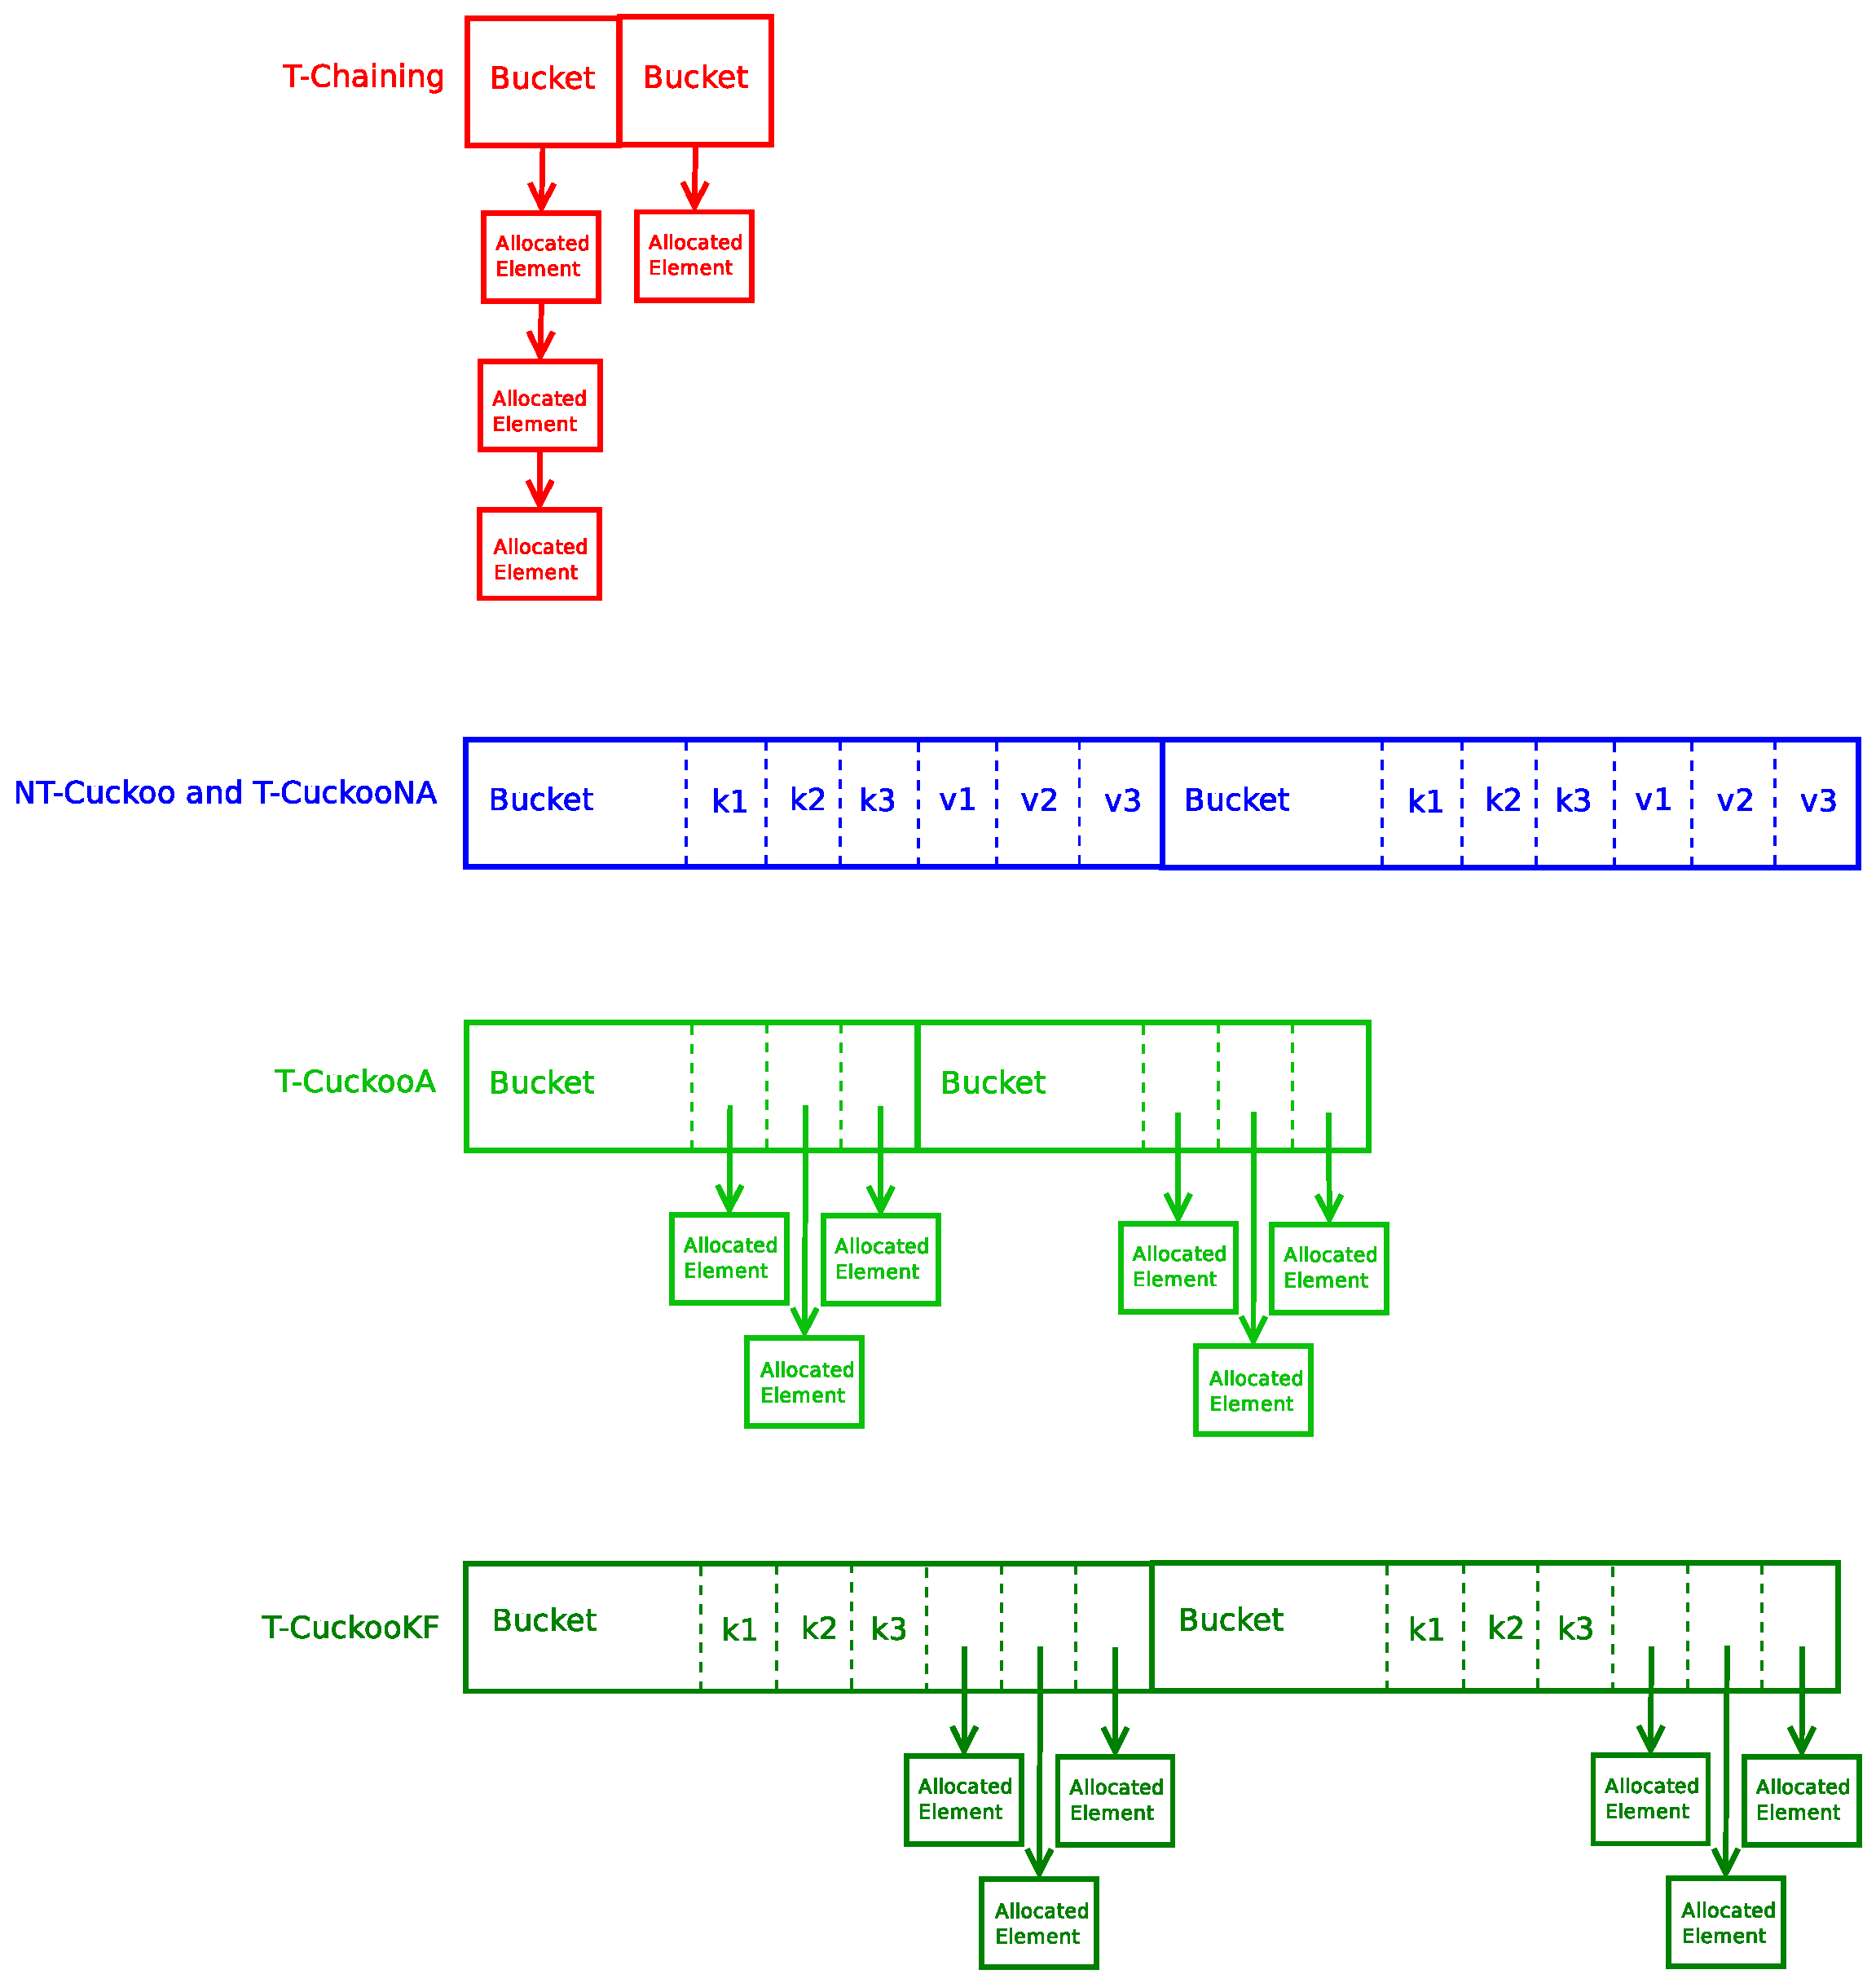
\includegraphics[width=0.9\textwidth]{hashmap_finds}
    \caption[Bucket Structure of Different Hashmaps]{This figure depicts two buckets in each type of hashmap. The static size of a bucket in each cuckoo hashmap is set to 3. Arrows represent pointers to allocated elements; contiguous memory is represented horizontally.}
\label{fig:hashmap_buckets}
\end{figure}

\subsection{Transactional Chaining Hashmap}
The transactional chaining hashmap is a concurrent, transactional hashmap implemented using a standard chaining algorithm. If two elements are mapped to the same bucket, they are chained in a linked list, shown in Figure~\ref{fig:hashmap_buckets} (a). Thus, the worst case time complexity for a lookup, insert, or delete is $O(n)$. Inserts require allocating an element corresponding to the inserted key-value pair to insert into the bucket. Each bucket is associated with a \emph{bucket version} that increments upon any committed addition or removal from the bucket. The bucket version is used to verify that no thread has added an element that was absent during a transaction's find. In addition, each bucket has a lock that synchronizes access to the bucket. Each inserted element is associated with an \emph{element version} that tracks if the value of the element has been modified or if the element has been removed. Each element version is tied to the inserted element's memory address.

Elements are inserted eagerly at execution time with a \emph{phantom} flag, allowing another transaction that sees ones of these uninstalled elements to realize it is viewing an inconsistent state of the map and therefore abort. If a transaction that performs an insertion later aborts, these phantom elements are removed from the map. Otherwise, the phantom mark is erased during commit. An alternative approach would be to insert all elements at commit time. However, this requires either relying on the bucket version to determine if another transaction has inserted the same element (which would result in false aborts since the bucket version increments for \emph{any} inserted value), or redoing the search for the element to see if the insertion can still occur. Thus, we insert at execution time to allow for more fine-grained validation checks at commit time, and to reduce redundant computations. 

Erasures are delayed until commit time (an optimistic approach). The same logic as we used for inserted items does not apply here. We could also use a flag on the bucket that contained the element to indicate that a transaction performed an erase of the element at execution time, and that the bucket is in an inconsistent state; another thread, upon seeing the flag, would abort. However, this loses the per-element granularity of checks and causes false aborts. Thus, erasing elements at execution time would decrease the granularity of validation checks, rather than increase it (as was the case for inserting elements).
Delaying erasures until commit time requires careful handling of cases of \emph{read-my-writes}, such as deleting an element inserted in the same transaction.

\subsection{Non-Transactional Cuckoo Hashmap}
\label{section:ntchm_algo}
The Non-Transactional Cuckoo Hashmap (NT-Cuckoo) implements a concurrent, non-transactional cuckoo hashing algorithm. We modify an implementation of a dynamically-resizing, concurrent cuckoo hashmap~\cite{cuckoocode} by simplifying several procedures; the main difference is that our cuckoo hashmap is statically sized.

We choose the cuckoo hashing algorithm as a potential transactional algorithm because the cuckoo hashing algorithm has several advantages over a chaining one. For one, cuckoo hashmaps have been shown to outperform chaining hashmaps when the hashmap can mostly fit in cache. Although cuckoo hashing has the disadvantage of performing two memory accesses for a lookup (as described below), the overhead from performing memory accesses is eliminated when the map can fit in cache.
Furthermore, modern processors can optimize these memory accesses to alleviate some of the overhead~\cite{chm_arch}.
Cuckoo hashmaps with large bucket sizes also outperform chaining hashmaps at high loads (when the average number of elements per bucket is high)~\cite{chm_load}. As we explain below, this is because the cost of a lookup is always constant time, whereas a chaining hashmap may experience $O(n)$ lookup time. In addition, a lookup that encounters a long chain in a chaining hashmap will follow $O(n)$ pointers, whereas a lookup in a cuckoo hashmap will need to only access two buckets, each of which is a contiguous array in memory.

In a concurrent setting, both cuckoo and chaining hashmaps must synchronize access to buckets. Because the granularity of synchronization is no different for the two algorithms, concurrent cuckoo hashing is still expected to outperform chaining for the same reasons (better cache usage due to lack of pointers, and improved asymptotic time complexity for all operations).

The cuckoo hashing algorithm works as follows: each element is placed in one of two buckets; these buckets are determined by two different hash functions. A bucket has a fixed size of elements. This means that lookups and deletes only require executing two hash functions and checking the contents of two buckets (an $O(1)$ operation).

Inserts run in amortized $O(1)$ time; the running time may occasionally be $O(n)$.
If an element $e$ is hashed by the first hash function to a bucket that is already full, the algorithm attempts to place $e$ in its alternate bucket by hashing $e$ with the second hash function. If both buckets are full, cuckoo shuffling occurs. This process evicts an element $e'$ in one of $e$'s buckets and places $e'$ in $e'$'s alternate bucket. If $e'$'s alternate bucket is full, an element $e''$ is ejected from this bucket, and so on. As long as the cuckoo shuffling does not encounter a bucket cycle, $e$ can now be placed in one of its buckets, as the removal of $e'$ has made space for $e$.
However, if the shuffling encounters a bucket cycle, the hashmap raises an \texttt{{out\_of\_space}} assertion error. We can imagine an alternative implementation that allows the hashmap to grow in number of buckets or otherwise change its hash functions, reinserting all elements, but for simplicity, we keep the hashmap statically sized.

Because the buckets are statically sized, elements are contained in fixed-size key and value arrays and therefore do not require extra allocations. The bucket structure is shown in Figure~\ref{fig:hashmap_buckets} (b). 

\subsection{Transactional Cuckoo Hashmap}

We hypothesize that, unlike the flat combining algorithm, the key optimizations of the cuckoo hashing algorithm---better cache usage at a high fullness and constant time (or amortized constant time) operations---are not crippled by integrating the algorithm into a transactional setting. This is because the modifications necessary to support transactions do not interfere with these optimizations taken by cuckoo hashing. We investigate this further in our evaluation (Section~\ref{hm_eval}) and hashmap dependencies discussion (Section~\ref{hm_deps}).

The transactional cuckoo hashmap comes in three flavors: two that allocate an element per insertion, and one that does not perform any allocations. All cuckoo hashmaps instrument the non-transactional cuckoo hashmap with STO calls that provide transactional guarantees.
Both allocating and non-allocating versions use the same synchronization algorithm: like the chaining hashmap, each bucket has a \emph{bucket version} and lock, and each element has an \emph{element version}. Because insertions can occur due to cuckoo shuffling as well as an external insertion call, the bucket version increments only when an element \emph{not already contained in the map} is inserted into the bucket (i.e., elements inserted via a call to insert and not via cuckoo shuffling). Elements are inserted at execution time with a \emph{phantom} flag that is then erased at commit time, and erasures are delayed until commit time.

The two variants of the allocating transactional cuckoo hashmap allocate elements upon insertion. One variant (T-CuckooA) consists of buckets containing pointers to the elements (Figure~\ref{fig:hashmap_buckets} (c)), allowing STO to track elements by their memory address to verify element versions at commit time. The key-fragments variant (T-CuckooKF) expands buckets to contain both an array of keys and an array of element pointers (Figure~\ref{fig:hashmap_buckets} (d)). This allows for a lookup to compare keys directly, because the keys are themselves contained in the bucket. Without the key-fragments, the lookup would have to follow pointers contained in the bucket to access and compare the key value. For many workloads, the key-fragments variant reduces the number of cache line accesses. STO can still track elements by their memory address in the element pointer array, but these pointers are only accessed if the value of the element is needed. This only happens during a present lookup, which accesses exactly one pointer, namely that of the searched-for element.

The non-allocating transactional cuckoo hashmap (T-CuckooNA) consists of buckets containing a fixed-sized array of elements (Figure~\ref{fig:hashmap_buckets} (b)). In this variant of the cuckoo hashmap, STO tracks elements by their keys rather than their memory address. Therefore, to verify if an element version has changed at commit time, the check procedure performs a find of the element using the key (searching at most two buckets) and validates the corresponding element version. Although this reduces the number of allocations, elements can now move between buckets and invalidate the values in the previous bucket: this greatly complicates the process of correctly checking and synchronizing element version reads. Our transactional algorithm for this hashmap reflects this complexity: the tracking set size is not minimal, and therefore we achieve more coarse-grained locking at commit time. For example, the non-allocating cuckoo hashmap locks both bucket versions to check any element version, because the element could move between buckets during the check. The allocating cuckoo hashmap needs only to lock the element version, because the hashmap has access to the element's unchanging memory address. 

Although a non-allocating transactional cuckoo hashmap is more complex, we build it to improve cache performance during lookups: the algorithm does not need to follow any pointers. Nonetheless, we may not see a great improvement in cache usage because we now must execute approximately double the number of lookups: each find requires performing two lookups (one during execution, and another during commit to check if the element version is still valid).


\section{Evaluation}
\label{hm_eval}

As we did with the queue, we evaluate all hashmaps on a set of microbenchmarks to determine their scalability and performance. We aim to provide evidence for our hypothesis that, unlike the flat combining queue, the cuckoo hashmap will retain its scalability and behavior even in a transactional setting.

\subsection{Microbenchmarks}
All experiments are run on the same machine as the queue experiments (with 100GB DRAM, two 6-core Intel Xeon X5690 processors with hyperthreading clocked at 3.47GHz and a 64-bit Linux 3.2.0 operating system). All benchmarks and STO data structures are compiled with \texttt{g++-5.3}. In all performance graphs, we show the median of 5 consecutive runs with the minimum and maximum performance results represented as error bars.
In all tests, threads are pinned to cores, with at most one thread per logical core.

Cache misses are recorded by running the benchmark with 8 threads, with each thread performing 9M transactions, under the profiling tool Performance Events for Linux (\texttt{perf}). The sampling period is set to 1000, meaning that every 1000th cache miss is recorded.
In the cache miss results presented, we report the number of cache misses reported by perf (approximately 1/1000 of the actual number of cache misses).

\subsubsection{Parameters}

    \emph{Proportion of Finds/Inserts/Deletes}. The ratio of inserts:deletes is kept at 1 to ensure that the hashmap does not always become empty or only grow in size. Keys are drawn uniformly at random from a predetermined range, in such a way that half of the inserts will succeed (the key to insert is not present) and half of the deletes will succeed (the key is present). Tests of 5\% inserts, 5\% deletes, and 90\% finds simulate the most likely use cases for hashmaps~\cite{hm1}. Tests of equal proportion (33\%) of all operations investigate how the hashmap reacts to an increased rate of inserts and deletes.

\emph{Operations per transaction}. We choose to run all tests comparing transactional to non-transactional (parallel-only) data structures using single-operation transactions. As discussed in Section~\ref{q_microbenchmarks}, this provides a more fair evaluation of transactional data structures against concurrent ones. In addition, it allows us to minimize the differences between transaction hashmap implementations so we can get a baseline comparison.

\emph{Number of buckets}. Both the cuckoo hashmaps and the chaining hashmap statically set the number of buckets in the data structure. The number of elements allowed in one bucket of the cuckoo hashmaps is fixed at a particular value, which we will call the \emph{maximum fullness}. 
        The \emph{capacity} (number of buckets $\times$ number of elements per bucket) of the cuckoo hashmap is fixed at some finite value because the cuckoo hashmap has a fixed size bucket; the chaining hashmap has no fixed capacity because a bucket's chain can grow arbitrarily long.
        The number of buckets and the size of each bucket affect the number of cache lines accessed during the test (for example, a larger hashmap may not be expected to fit into the L2 cache, whereas a small hashmap at full capacity will fit entirely in cache). During all tests, the number of keys present in the hashmap is not allowed to outgrow its capacity.
    
    \emph{Fullness}. Fullness indicates the ratio of the number of keys to the number of buckets. This determines the average number of elements to be found per bucket. The tests are implemented such that at steady state, fullness is expected to be 75\% of the maximum fullness of the cuckoo hashmap to avoid an out-of-space exception. This is controlled by picking a maximum key value. The maximum key value of inserted elements is twice the number of elements the hashmap will contain when its size reaches a fixed point.

        Note that the initial size of the data structure should not affect performance as the test proceeds for a longer period of time and reaches a steady state. Therefore, we do not include the initial size as a benchmark parameter.

\subsubsection{Multi-Thread, Variable-Capacity Singletons Test} 
This test is run with varying numbers of threads, in which each thread runs 5 million singleton transactions.
The test is run twice, once with a probability of 33\% insert, 33\% delete, and 34\% find, and again with a probability of 5\% insert, 5\% delete, and 90\% find. The steady-state final size is 75\% maximum fullness (of the cuckoo hashmap).

\subsection{Overview of Results}

We measure all the performance of all hashmaps in terms of operations per second, abort rates, and cache performance (number of cache misses). 
The full results can be found in Appendix~\ref{app:hashmaps}. As we did with the queue results, we proceed in our discussion by first giving an overview of our conclusions, then show how we reach these conclusions through a sequence of hypotheses.

Our results demonstrate the following:
\begin{itemize}
    \item The key-fragments transactional cuckoo hashmap achieves the best overall cache performance. The number of cache misses is strongly correlated with overall performance, particularly because the abort rate of our tests is negligible.
    \item When the hashmap can fit entirely or mostly in cache, the transactional cuckoo hashmaps outperform the transactional chaining hashmap.
    \item When the hashmap has a high maximum fullness, the transactional cuckoo hashmaps outperform the transactional chaining hashmap.
    \item The relative performance of the transactional cuckoo hashmaps and the transactional chaining hashmap mirrors the relative performance expected of their non-transactional counterparts.
\end{itemize}

\subsection{Hypothesis 1}
\subsubsection{The non-allocating transactional cuckoo hashmap (T-CuckooNA) achieves the best cache usage out of all transactional hashmaps (Not Supported).}
\label{section:hmcm}

The number of cache misses is influenced by the number of allocations, the patterns in which these allocations are accessed, and the patterns in which the hashmap buckets themselves are accessed. Our results in Figures~\ref{fig:hm_cm5},~\ref{fig:hm_cm10}, and~\ref{fig:hm_cm15} demonstrate that, as expected, a pattern of 90\% finds (5\% inserts/5\% erases) achieves better cache performance than a pattern of 33\% finds/inserts/erases.

    \begin{figure}[H]
    \centering
        \begin{minipage}{0.75\textwidth}
        \centering
            \boxed{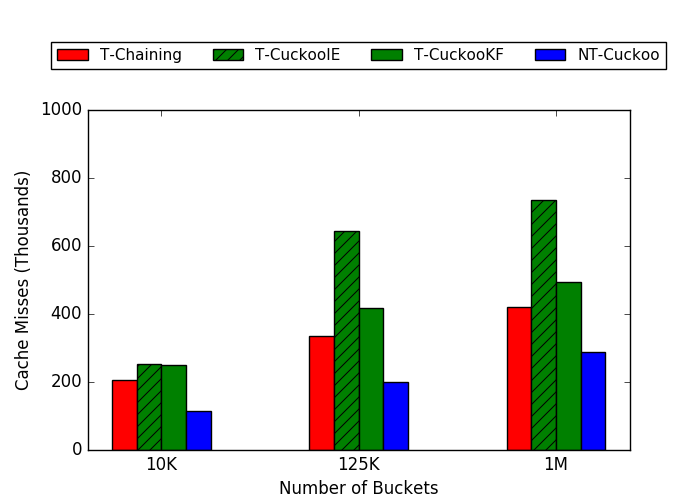
\includegraphics[width=\textwidth]{maps/335cm.png}}
            \caption*{33\%Find, 33\%Insert, 33\%Delete}
            \vspace{12pt}
        \end{minipage}
        \begin{minipage}{0.75\textwidth}
            \centering
            \boxed{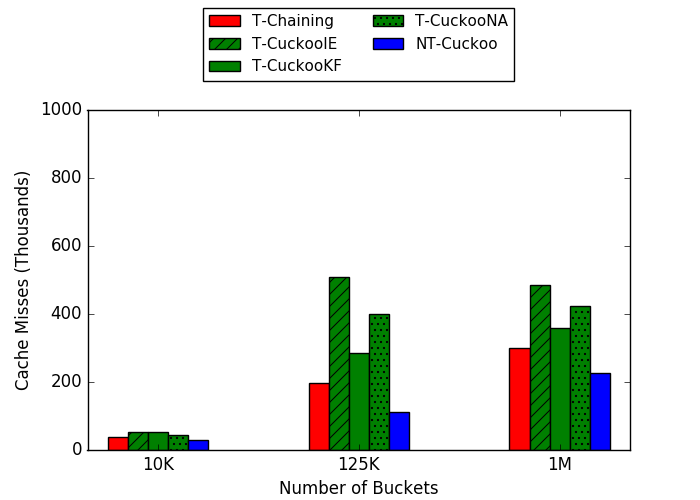
\includegraphics[width=\textwidth]{maps/905cm.png}}
            \caption*{90\%Find, 5\%Insert, 5\%Delete}
        \end{minipage}
        \caption[Hashmap Cache Misses (Max Fullness 5)]{Hashmap Cache Misses (Max Fullness 5): T-Chaining has the best cache performance of the transactional hashmaps.}
		\label{fig:hm_cm5}
    \end{figure}

    \begin{figure}[H]
    \centering
        \begin{minipage}{0.75\textwidth}
        \centering
            \boxed{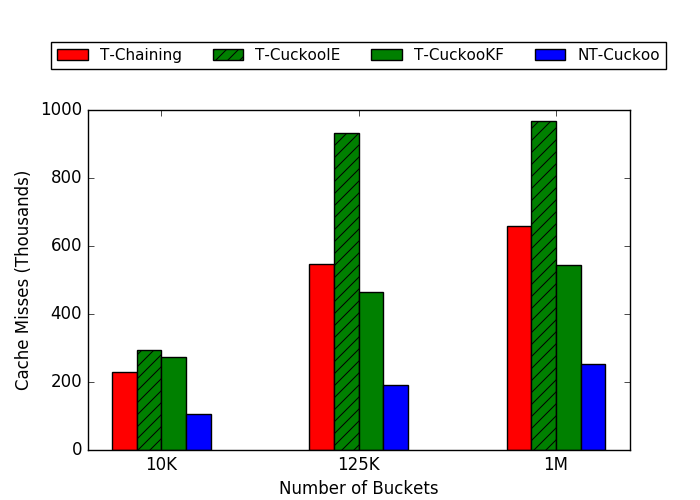
\includegraphics[width=\textwidth]{maps/3310cm.png}}
            \caption*{33\%Find, 33\%Insert, 33\%Delete}
            \vspace{12pt}
        \end{minipage}
        \begin{minipage}{0.75\textwidth}
            \centering
            \boxed{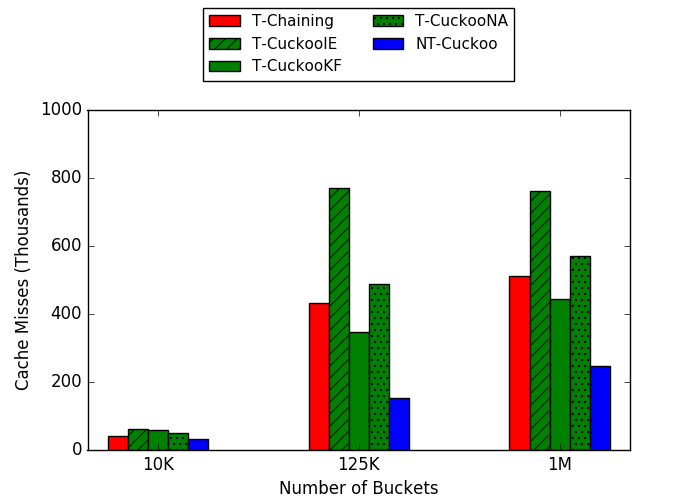
\includegraphics[width=\textwidth]{maps/9010cm.png}}
            \caption*{90\%Find, 5\%Insert, 5\%Delete}
        \end{minipage}
        \caption[Hashmap Cache Misses (Max Fullness 10)]{Hashmap Cache Misses (Max Fullness 10): T-CuckooKF has the best cache performance of the transactional hashmaps, followed by T-CuckooNA.}
		\label{fig:hm_cm10}
    \end{figure}

    \begin{figure}[H]
    \centering
        \begin{minipage}{0.75\textwidth}
        \centering
            \boxed{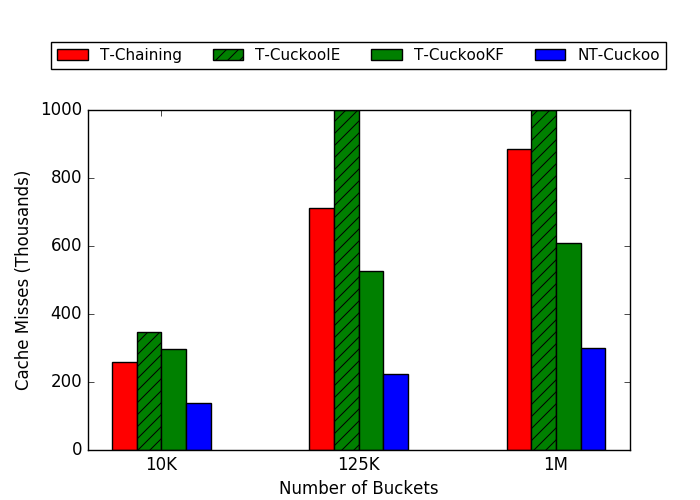
\includegraphics[width=\textwidth]{maps/3315cm.png}}
            \caption*{33\%Find, 33\%Insert, 33\%Delete}
            \vspace{12pt}
        \end{minipage}
        \begin{minipage}{0.75\textwidth}
            \centering
            \boxed{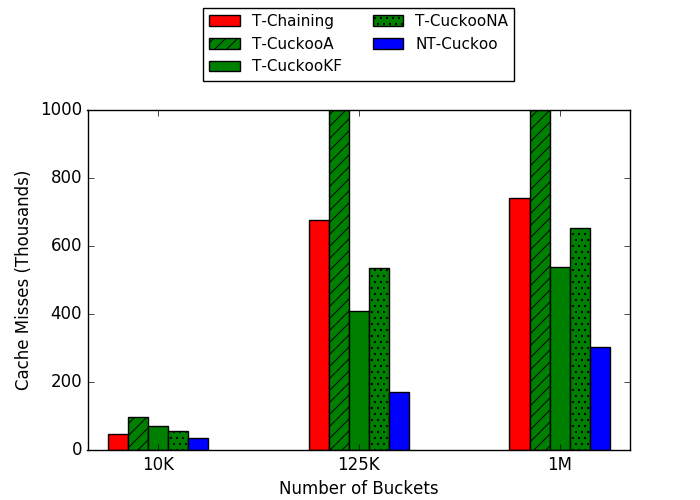
\includegraphics[width=\textwidth]{maps/9015cm.png}}
            \caption*{90\%Find, 5\%Insert, 5\%Delete}
        \end{minipage}
        \caption[Hashmap Cache Misses (Max Fullness 15)]{Hashmap Cache Misses (Max Fullness 15): T-CuckooKF has the best cache performance of the transactional hashmaps, followed by T-CuckooNA. We see that the difference between T-CuckooKF's cache performance and T-Chaining's cache performance is increasing as fullness increases.}
		\label{fig:hm_cm15}
    \end{figure}

The non-transactional cuckoo hashmap experiences the least number of cache misses on all tests, which we expect given its lack of transactional instrumentation. Somewhat surprisingly, the non-allocating, transactional cuckoo hashmap does not achieve the best overall cache performance. 
As we see in Figure~\ref{fig:hm_cm5}, T-Chaining has the best cache performance among the transactional hashmaps when the maximum fullness (i.e., the maximum load on the hashmap) is set to 5. This is likely due to the low number of element pointer accesses when T-Chaining performs a find: the chains are relatively short, and an absent find requires following no pointers. 
In comparison, the cuckoo hashmaps must search through two entire bucket arrays on an absent find. 

Figures~\ref{fig:hm_cm10} and~\ref{fig:hm_cm15} indicate that when the hashmap has longer chains or bucket sizes (maximum fullness 10 or 15) and cannot fit entirely in cache (i.e., the number of buckets is 125K or 1M), T-CuckooKF achieves the best transactional hashmap cache performance, followed by T-CuckooNA. 
The difference in the number of cache misses between T-Chaining and T-CuckooKF increases as maximum fullness increases; this occurs because T-Chaining, on average, has to follow more pointers each time it performs a lookup, because the chain lengths are longer on average.
T-Chaining and T-CuckooA experienced a decrease in cache performance in these scenarios because a find will not need to follow pointers in the buckets of either T-CuckooKF or T-CuckooNA, whereas every find in T-Chaining and T-CuckooA requires following pointers. As the maximum fullness increases, T-CuckooA and T-Chaining maps follow an increasing number of pointers per find.
We conjecture that T-CuckooKF has fewer cache misses than T-CuckooNA because the additional memory accesses from following pointers is minimal (a present find follows only one pointer), and the additional lookups in T-CuckooNA mean that T-CuckooNA accesses approximately twice the number of buckets per operation compared to T-CuckooKF.

\vspace{12pt}
\noindent\fbox{\begin{minipage}{\textwidth}
    \textbf{NOT SUPPORTED}: T-CuckooNA has worse cache performance than T-CuckooKF when the hashmap has 125K or 1M buckets, and only slightly better cache performance when the hashmap has 10K buckets. When chains are short (fullness is 5), T-Chaining has the best cache performance.
\end{minipage}}

\subsection{Hypothesis 2}
\subsubsection{When the hashmap can fit entirely or mostly in cache, the transactional cuckoo hashmaps outperform the transactional chaining hashmap (Supported).}

\begin{figure}[ht!]
    \centering
    \begin{minipage}{0.75\textwidth}\boxed{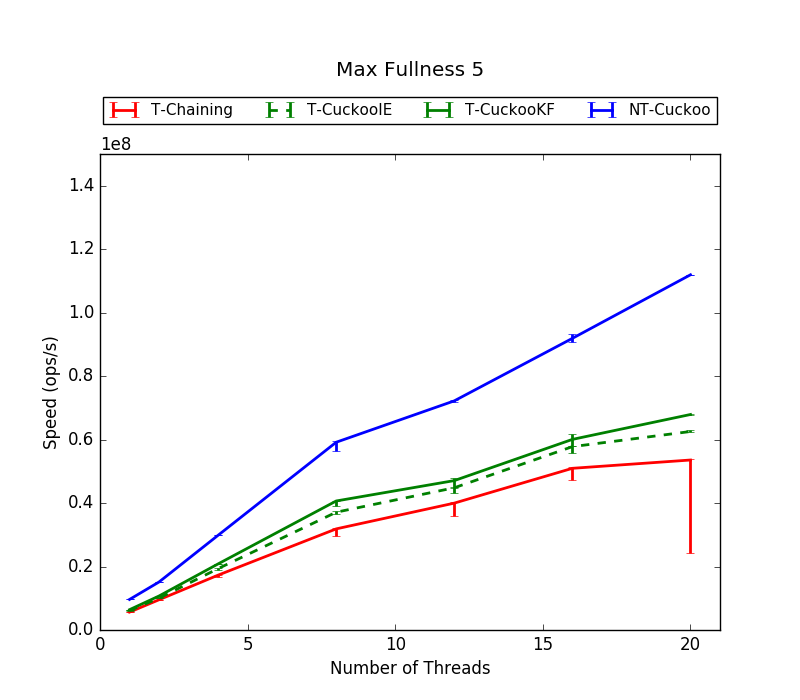
\includegraphics[width=\textwidth]{maps/5HM10K:F90,I5,E5.png}}
	\caption*{90F/5I/5E}
        \vspace{12pt}
    \end{minipage}
    \begin{minipage}{0.75\textwidth}\boxed{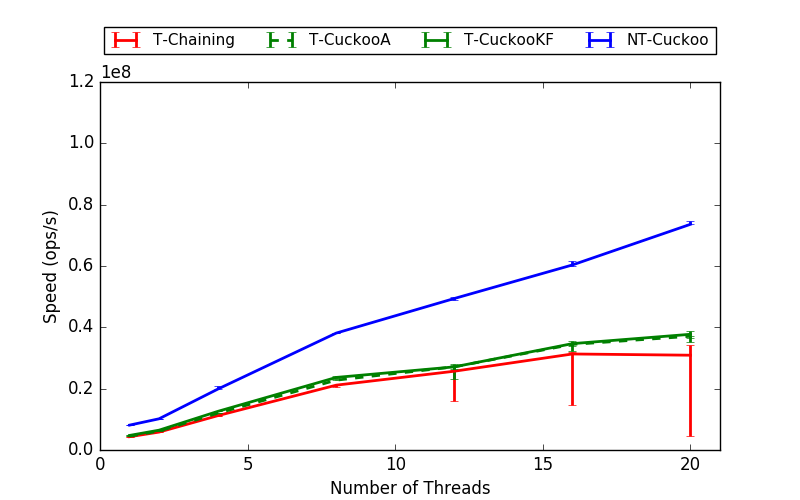
\includegraphics[width=\textwidth]{maps/5HM10K:F34,I33,E33.png}}
	\caption*{33F/33I/33E}
    \end{minipage}
    \caption[Hashmap Performance: 10K Buckets, Maximum Fullness 5]{Hashmap Performance: 10K Buckets, Maximum Fullness 5. The transactional cuckoo hashmaps outperform T-Chaining.}
    \label{fig:hm_5}
\end{figure}


To evaluate this hypothesis, we look at our results for a map with 10K buckets with a low maximum fullness of 5, which fits entirely in cache (Figure~\ref{fig:hm_5}).\footnote{Our preliminary performance results on the Multi-thread Singletons Test show the same pattern as our cache performance results: T-CuckooNA performs better than T-CuckooA on average and worse than T-CuckooKF. We omit these results from our performance results presented here because the correctness of T-CuckooNA implementation has not been confirmed.}
For all hashmaps, performance with 90\% finds (5\% inserts/erases) is approximately $1.5\times$ that of the 33\% finds/inserts/erases. This is expected: a find is both faster to perform than an insert or delete, and a find requires only reading a bucket version for all transactional hashmaps.
On both benchmarks, the cuckoo hashmaps achieve performance approximately $1.2\times$ that of T-Chaining. There is little difference between the performance of T-CuckooA and the performance of T-CuckooKF, because cache performance does not play a significant role in these benchmarks.

We note that this result is consistent with the claim made in Section~\ref{section:ntchm_algo} that cuckoo hashmaps outperform chaining hashmaps when the hashmap can fit in cache. 

\vspace{12pt}
\noindent\fbox{\begin{minipage}{\textwidth}
    \textbf{SUPPORTED}: The transactional cuckoo hashmaps outperform the transactional chaining hashmap when the hashmap can fit in cache.
\end{minipage}}

\subsection{Hypothesis 3}
\subsubsection{As maximum fullness increases, T-CuckooKF outperforms T-Chaining by a greater margin (Supported).}

\begin{figure}[ht!]
    \centering
    \begin{minipage}{0.7\textwidth}\boxed{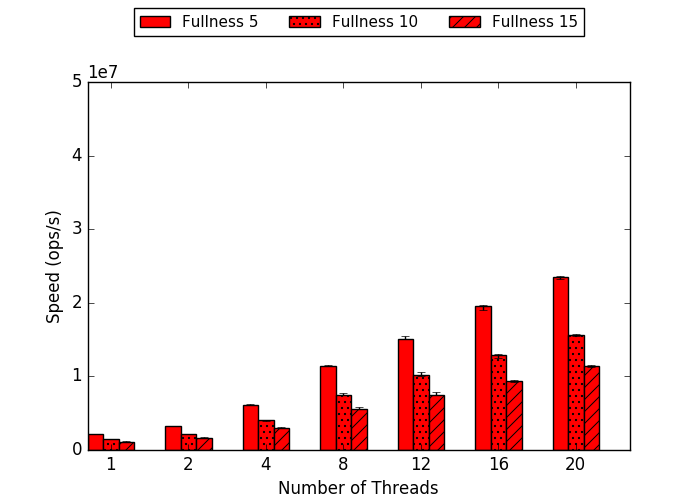
\includegraphics[width=\textwidth]{maps/chainingHM1M:F34,I33,E33_fullness.png}}
    \caption*{T-Chaining}
        \vspace{12pt}
    \end{minipage}
    \begin{minipage}{0.7\textwidth}\boxed{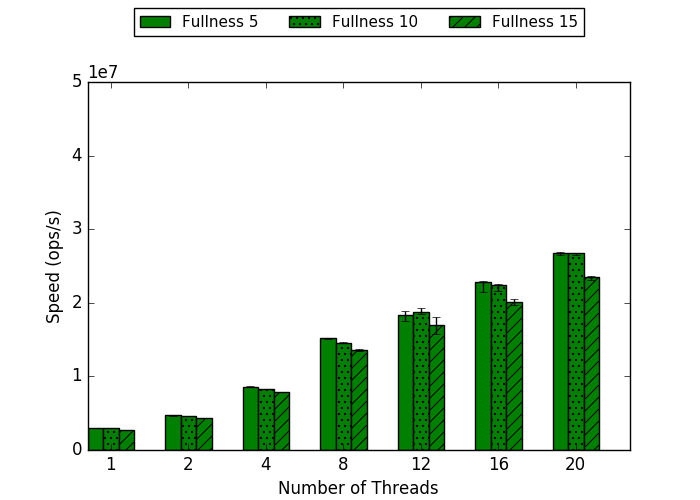
\includegraphics[width=\textwidth]{maps/kfHM1M:F34,I33,E33_fullness.png}}
    \caption*{T-CuckooKF}
    \end{minipage}
    \caption[T-Chaining vs. T-CuckooKF: Performance as fullness increases (1M Buckets, 33F/33I/33E)]{T-Chaining vs. T-CuckooKF: Performance as fullness increases (1M Buckets, 33F/33I/33E). T-Chaining experiences a greater drop in performance than does T-CuckooKF as fullness increases. T-Chaining's performance drops over 50\% as fullness goes from 5 to 15.}
    \label{fig:hm_fullness_33_2}
\end{figure}

\begin{figure}[ht!]
    \centering
    \begin{minipage}{0.70\textwidth}\boxed{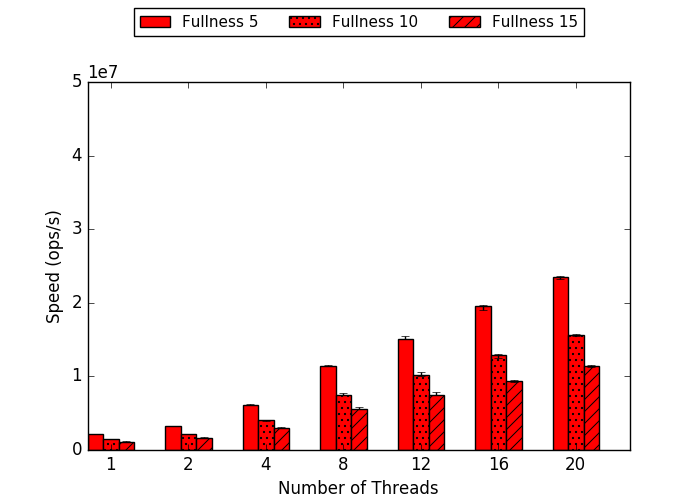
\includegraphics[width=\textwidth]{maps/chainingHM1M:F34,I33,E33_fullness.png}}
    \caption*{T-Chaining}
        \vspace{12pt}
    \end{minipage}
    \begin{minipage}{0.70\textwidth}\boxed{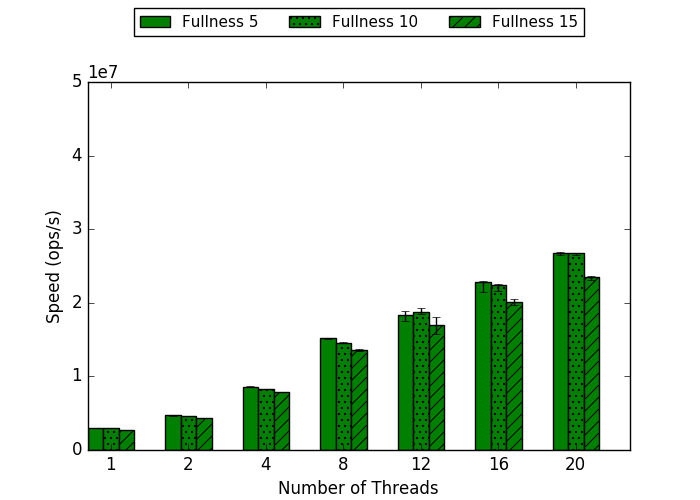
\includegraphics[width=\textwidth]{maps/kfHM1M:F34,I33,E33_fullness.png}}
    \caption*{T-CuckooKF}
    \end{minipage}
    \caption[T-Chaining vs. T-CuckooKF: Performance as fullness increases (1M Buckets, 90F/5I/5E)]{T-Chaining vs. T-CuckooKF: Performance as fullness increases (10K Buckets, 90F/5I/5E). T-Chaining experiences a greater drop in performance than does T-CuckooKF as fullness increases. T-Chaining's performance decreases by over 50\% with 1M buckets as fullness increases.}
    \label{fig:hm_fullness_90_2}
\end{figure}

We analyze our results for maps with various number of buckets and compare their performance with a high maximum fullness of 5 to that with a maximum fullness of 15. We show the results for maps with 1M buckets (full results are in Appendix~\ref{app:hashmaps}).

We first consider the results from the 33\% finds/inserts/erases test. Our results show that T-CuckooKF achieves performance $1.5$--$2\times$ that of T-Chaining as maximum fullness increases to 15, regardless of the number of buckets (Figure~\ref{fig:hm_fullness_33_2}). 
This is caused by a decrease in the performance of T-Chaining as fullness increases. Performance decreases by approximately 33\% when the hashmap has 10K buckets, and by over 50\% when the hashmap has 1M buckets (Figure~\ref{fig:hm_fullness_33_2}). T-CuckooKF's performance, in contrast, decreases only slightly or remains essentially unchanged.

Our results from the 33\% finds/inserts/erases test therefore support our hypothesis regardless of the number of buckets in the hashmap: the difference between T-CuckooKF's performance and T-Chaining's performance increases as fullness increases. 

We also consider our results from the 90\% finds (5\% inserts/erases) test to see if they support our hypothesis.
Again, fullness seems to have a drastic impact on T-Chaining's performance regardless of the number of buckets in the hashmap (performance drops by approximately 50\%) and almost no impact on the performance of T-CuckooKF (Figure~\ref{fig:hm_fullness_90_2}). 

When the hashmap contains 10K buckets, T-CuckooKF's performance is approximately $1.2\times$ that of T-Chaining at a fullness of 5. This difference increases with fullness: T-CuckooKF performs over $2\times$ better than T-Chaining at a fullness of 15.
We observe a similar phenomenon when the map has 125K buckets and 1M buckets (Figure~\ref{fig:hm_fullness_90_2}): T-CuckooKF's performance goes from approximately $2\times$ the performance of T-Chaining at a fullness of 5, to over $3\times$ at a fullness of 15.
 
This result is consistent with the claim made in Section~\ref{section:ntchm_algo} that cuckoo hashmaps outperform chaining hashmaps when the average number of elements per bucket (fullness) is high.
Regardless of the number of buckets in the map, T-Chaining experiences a much more drastic drop in performance than T-CuckooKF as fullness increases, and the difference in performance therefore increases.

\vspace{12pt}
\noindent\fbox{\begin{minipage}{\textwidth}
    \textbf{SUPPORTED}: T-CuckooKF outperforms T-Chaining by a greater margin as maximum fullness increases.
\end{minipage}}


\subsection{Hypothesis 4}
\subsubsection{An algorithm's cache usage most heavily affects performance on our benchmarks; abort rate has a negligible effect on performance (Supported).}

    We pose this hypothesis to determine if the bottleneck in performance is the algorithm's cache usage or its abort rate. 
Our results for both tests discussed in Hypothesis 3 indicate that the number of cache misses is strongly correlated with performance. In general, the performance of all hashmaps decreases slightly (less than 20\%) as hashmap size increases from 10K to 1M buckets. We attribute this to the increasing number of cache misses with increasing numbers of buckets.

The greater difference between T-CuckooKF's performance and T-Chaining's performance as fullness increases is also mirrored in the increased difference between T-CuckooKF's and T-Chaining's number of cache misses (discussed in Section~\ref{section:hmcm}). T-CuckooA's performance also drops more significantly than T-CuckooKF's as fullness increases (we observe, however, that T-CuckooA still performs at least as well as T-Chaining). T-CuckooA uses the same algorithm as T-CuckooKF, but has worse cache usage, which provides further evidence that cache usage plays a crucial part in performance. 

    \begin{table}[t]
    \centering
	\singlespace
        \begin{minipage}{\textwidth}
            \centering
        \begin{tabular}{|c|c|c|c|}
\hline
\multirow{2}{*}{Hashmap} & \multicolumn{3}{c|}{\#Threads Abort Rate (\%)}\\\cline{2-4}& 4 & 12 & 20\\
\hline
\hline
T-Chaining & 0.003 & 0.013 & 0.021\\
T-CuckooIE & 0.001 & 0.004 & 0.005\\
T-CuckooKF & 0.001 & 0.004 & 0.007\\
NT-Cuckoo & 0.000 & 0.000 & 0.000\\
\hline
\end{tabular}

        \caption*{10K Buckets}
            \vspace{12pt}
        \end{minipage}
        \begin{minipage}{\textwidth}
            \centering
        \begin{tabular}{|c|c|c|c|}
\hline
\multirow{2}{*}{Hashmap} & \multicolumn{3}{c|}{\#Threads}\\\cline{2-4}& 4 & 12 & 20\\
\hline
\hline
T-Chaining & 0.000 & 0.002 & 0.002\\
T-CuckooIE & 0.000 & 0.000 & 0.001\\
T-CuckooKF & 0.000 & 0.000 & 0.001\\
NT-Cuckoo & 0.000 & 0.000 & 0.000\\
\hline
\end{tabular}

        \caption*{125K Buckets}
        \end{minipage}
        \caption{Hashmap Abort Rate (Max Fullness 10, 33\% Finds/Inserts/Erases)}
		\label{tab:hm_aborts}
    \end{table}

    Our results in Table~\ref{tab:hm_aborts} and in Appendix~\ref{app:hm_aborts} indicate that the abort rate remains relatively constant regardless of the fullness of the hashmap, but decreases as the number of buckets in the map increases. A greater number of buckets decreases the abort rates, since the probability that two threads will simultaneously attempt to read or modify the same bucket decreases. Abort rate is negligible in nearly all tests, with the chaining hashmap experiencing the highest abort rates (the median of 5 trials never exceeding 0.006\%).

We see that cache performance affects overall performance more than the abort rate; as the number of buckets increases, performance drops even while the abort rate decreases. The major factor detracting from performance appears to be the significant increase in the number of cache misses.

\vspace{12pt}
\noindent\fbox{\begin{minipage}{\textwidth}
    \textbf{SUPPORTED}: The number of cache misses is strongly correlated with performance, but abort rate does not heavily affect performance.
\end{minipage}}

\subsection{Conclusion}

Our evaluation demonstrates that the cuckoo hashmap does not experience crippling performance loss when integrated into a transactional setting, and that a scalable, yet transactional, cuckoo hashmap implementation exists. Furthermore, the relative behavior of the transactional cuckoo and chaining hashmap mirrors the expected behavior of their non-transactional counterparts: the cuckoo hashmap also outperforms the transaction chaining hashmap in scenarios in which cache performance is a bottleneck (high fullness), or when the time complexity and time to execute the operations is a bottleneck (when the hashmap can fit in cache). 

We contrast our results with that of the strong transactional flat combining queue and note that, unlike the strong flat combining queue, the cuckoo (and chaining) hashmaps scale in a transactional setting. We now look to the scalable commutativity rule, and the commutativity of our hashmap interface, to determine exactly why our transactional hashmaps can scale when our strong transactional queues cannot. 

\section{Commutativity of Transactional Hashmaps}
\label{hm_deps}

In this section, we discuss the commutativity of non-transactional and transactional hashmap operations. We argue that synchronizing non-commutative transactions does not cripple the scalability of hashmaps implementing our hashmap interface, and that this occurs because the transactional setting adds few additional commutativity constraints to our hashmap interface. This is exemplified by our transactional chaining or cuckoo hashmap algorithms, which both scale in a transactional setting. 

Our commutativity and scalability results with cuckoo and chaining hashmaps are in sharp contrast with our results from the strong flat combining queue. In Chapter~\ref{commutativity}, we saw how the flat combining technique relies on operation commutativity that is heavily reduced in a transactional setting, and that the modifications to flat combining required to synchronize non-commuting transactions reduce the effectiveness of the flat combining technique and cripple its scalability. 
As we discover, the hashmap interface experiences only a slight loss of operation commutativity in a transactional setting; this allows transactional cuckoo and chaining hashing algorithms to scale.

In a non-transactional hashmap, insert and erase operations do not commute with finds, other inserts, or other erases when both (1) the same key is used as an argument or the argument keys collide by being hashed to the same bucket, and (2) at least one insert or delete succeeds.
    These are shown in Table~\ref{tab:hm_commute}. Both cuckoo and chaining hashmaps synchronize these non-commutative operations with per-bucket locks: an insert or erase in a chaining hashmap acquires a bucket-specific lock that protects access to the bucket during the duration of the insert or delete, while an insert or erase in a cuckoo hashmap locks both buckets in which the element may be placed. If the hashmap is large and if the workload uses a large range of keys, it is very likely that two operations will commute because they will modify or read separate buckets.
By the scalable commutativity rule, there exists a implementation of a hashmap algorithm that scales whenever insert or erase operations occur in separate buckets. Indeed, there are several examples of non-transactional chaining and cuckoo hashmap implementations that scale (with most reasonable hashmap workloads and a large enough map).

\begin{table}[t]
    \singlespace
    \centering
    \begin{tabular}{|c|l|l|}
        \hline
        Operations & \multicolumn{1}{c}{H} & \multicolumn{1}{|c|}{H'} \\
        \hline
    
        insert vs. erase &
\begin{lstlisting}
(T, M.insert(k,v), false)                       
(T, M.erase(k), true)
\end{lstlisting} &
\begin{lstlisting}
(T, M.erase(k), true)
(T, M.insert(k,v), true)                       
\end{lstlisting}\\
\hline
    insert vs. find &
\begin{lstlisting}
(T, M.insert(k,v), true)                       
(T, M.find(k,v), true)
\end{lstlisting} &
\begin{lstlisting}
(T, M.find(k,v), false)
(T, M.insert(k,v), true)                       
\end{lstlisting}\\
    \hline
   erase vs. find&
\begin{lstlisting}
(T, M.erase(k), true)                       
(T, M.find(k,v), false)
\end{lstlisting} &
\begin{lstlisting}
(T, M.find(k,v), true)                       
(T, M.erase(k), true)
\end{lstlisting}\\
    \hline
    insert vs. insert &
\begin{lstlisting}
(T1, M.insert(k,v), true)                       
(T2, M.insert(k,v), false)
\end{lstlisting} &
\begin{lstlisting}
(T2, M.insert(k,v), true)
(T1, M.insert(k,v), false)                       
\end{lstlisting}\\
\hline
     erase vs. erase&
\begin{lstlisting}
(T1, M.erase(k), true)                       
(T2, M.erase(k), false)
\end{lstlisting} &
\begin{lstlisting}
(T2, M.erase(k), true)                       
(T1, M.erase(k), false)
\end{lstlisting}\\
\hline    
    \end{tabular}
    \caption[Hashmap operations that do not commute]{Hashmap operations that do not commute. H is the original history; H' is the history with the order of the two operations exchanged. In the last two scenarios, note that it is important that the operations be performed by two different threads for there to be different observable results in the history.}
    \label{tab:hm_commute}
    \end{table}

In a transactional setting, we have the added constraint that no two transactions commute if exchanging the order of of the two transactions means that (a) any operation in one transaction observes that a key is present given one order, but not the other; and/or (b) the presence of any key in the map immediately after both transactions have committed in the history is different in one order from the resulting size in the other.

We can reason about commutativity in a transactional setting in terms of \emph{sets} of buckets that overlap between two transactions, rather than individual buckets that are both modified/read by two operations. If an operation in a transaction modifies a bucket that is read or modified by an operation in another transaction, then the two transactions will not commute.
Examples of larger transactions that fail to commute are shown in Table~\ref{tab:txnal_hm_commute}.

As in the non-transactional setting, if the hashmap is large and if the workload uses a large range of keys, it is very likely that two transactions will commute because they will modify or read separate sets of buckets. 
The intersection between the set of buckets modified in one transaction, and the set of buckets modified in the other, is likely to be empty or small (depending on the length of the transactions and the particular workload). We can therefore expect that an implementation of a cuckoo or chaining hashmap will still scale in a transactional setting in nearly all the same scenarios in which individual operations commute. 

\begin{table}[t]
    \singlespace
    \centering
    \begin{tabular}{|c|l|l|}
        \hline
        Example & \multicolumn{1}{c}{H} & \multicolumn{1}{|c|}{H'} \\
        \hline
        1.     &
\begin{lstlisting}
(T1, START_TXN, ())                       
(T1, M.find(k1,v), false)
(T1, M.insert(k1,v), true)                       
(T1, M.insert(k2,v), true)                       
(T1, COMMIT_TXN, ())                       
(T2, START_TXN, ())                       
(T2, M.find(k1,v), true)
(T2, M.insert(k1,v), false)
(T2, M.find(k2,v), true)
(T2, COMMIT_TXN, ())                       
\end{lstlisting} &
\begin{lstlisting}
(T2, START_TXN, ())                       
(T2, M.find(k1,v), false)
(T2, M.insert(k1,v), true)
(T2, M.find(k2,v), false)
(T2, COMMIT_TXN, ())                       
(T1, START_TXN, ())                       
(T1, M.find(k1,v), true)
(T1, M.insert(k1,v), false)                       
(T1, M.insert(k2,v), true)                       
(T1, COMMIT_TXN, ())                       
\end{lstlisting}\\
\hline
        2. &
\begin{lstlisting}
(T1, START_TXN, ())                       
(T1, M.erase(k1), false)                       
(T1, M.erase(k2), true)
(T1, M.insert(k2,v), true)                       
(T1, COMMIT_TXN, ())                       
(T2, START_TXN, ())                       
(T2, M.insert(k1,v), true)
(T2, M.insert(k2,v), false)
(T2, COMMIT_TXN, ())                       
\end{lstlisting} &
\begin{lstlisting}
(T2, START_TXN, ())                       
(T2, M.insert(k1,v), true)
(T2, M.insert(k2,v), false)
(T2, COMMIT_TXN, ())                       
(T1, START_TXN, ())                       
(T1, M.erase(k1), true)                       
(T1, M.erase(k2), true)
(T1, M.insert(k2,v), true)                       
(T1, COMMIT_TXN, ())                       
\end{lstlisting}\\
\hline    
    \end{tabular}
    \caption[Example hashmap transactions that do not commute]{Example hashmap transactions that do not commute. H is the original serial history; H' is the history with the order of the two transactions exchanged.}
    \label{tab:txnal_hm_commute}
    \end{table}

To synchronize transactions that do not commute, both the cuckoo and chaining hashmaps must synchronize all buckets that are modified by both transactions, or that are modified by one transaction and observed by another. We note that the synchronization necessary to add transactional guarantees to the cuckoo hashmap is essentially equivalent to those necessary to add transactional guarantees to the chaining hashmap. The difference between two synchronization mechanisms is that an operation that will require synchronizing one bucket in the chaining hashmap will instead require synchronizing two buckets in the cuckoo hashmap. The method in which transactions are synchronized is as follows:

A transactional find in a cuckoo hashmap and a chaining hashmap adds to the read set an object representing the bucket(s) in which the object should be (or is) located. A transactional insert adds a read of the bucket in which the key is located only if the key is already present; and a transactional erase adds a read of the bucket(s) in which the key is located if the key is absent, or a write of the bucket(s) if the key to erase is present. At commit time, any buckets that are read are locked; the reads are then checked, and the writes installed.

We note that buckets are locked only at execution time, only at commit time, or at both commit and execution time, depending on which operation accesses the buckets. A transactional find, unsuccessful erase, or unsuccessful insert locks the appropriate buckets only at commit time. A successful transactional erase locks the appropriate buckets only at commit time, and a successful transactional insert locks the appropriate buckets only at execution time (a bucket in which an element is inserted at execution time does not need to be locked at commit time because insertions are eager).

This algorithm allows for a implementation of a transactional hashmap that can scale in nearly all those scenarios in which an implementation of a non-transactional hashmap can scale. This is because the granularity of synchronization of the transactional hashmap is still per-bucket synchronization. 
The synchronization schemes of the cuckoo and chaining hashmaps rely on the fundamental assumption that operations performed on separate buckets will commute with each other. In a transactional setting, this assumption is still true for transactions whose operations modify or read on disjoint sets of buckets. Because the scenarios that require extra synchronization to handle non-commuting transactions are rare, and these scenarios do not require synchronization beyond the level of buckets, both the transactional cuckoo and chaining hashmaps scale in nearly all the same situations in which their non-transactional counterparts scale. 
This demonstrates that, unlike our queue operation interface, our hashmap operation interface (and the commutativity of operations in a transactional setting) allows for a scalable implementation of a transactional hashmap.

Furthermore, the cuckoo hashmap retains its non-transactional characteristics of better cache performance than the chaining hashmap, and asymptotic constant (or amortized constant) time bounds for its operations, even in the transactional setting. This is because the fundamental aspects of the algorithm---hashing into multiple buckets of fixed size, and the cuckoo hashing scheme for inserts---is not modified when the cuckoo hashmap is made transactional. As we stated earlier, this result contrasts with our findings with the flat combining algorithm, which has to be fundamentally modified to support queue transactions.

